%\pagebreak

\subsection{Evidencia de realizaci\'on}
Las figuras 1 y 2 muestran los objetos escaneados ya con los puntos de identificaci\'on. La figura 3, la
computadora empleada para el escaneo. Las figuras 4 y 5 contienen las superficies obtenidas despu\'es del
escaneo.\\

Tambi\'en se provee el hiperv\'inculo para descargar los archivos de la pr\'actica:
\begin{itemize}
 \item https://github.com/der-coder/materialsScience/tree/master/reporte3D/DreamTeam
\end{itemize}


 \begin{figure}[!htbp]
 \centering
 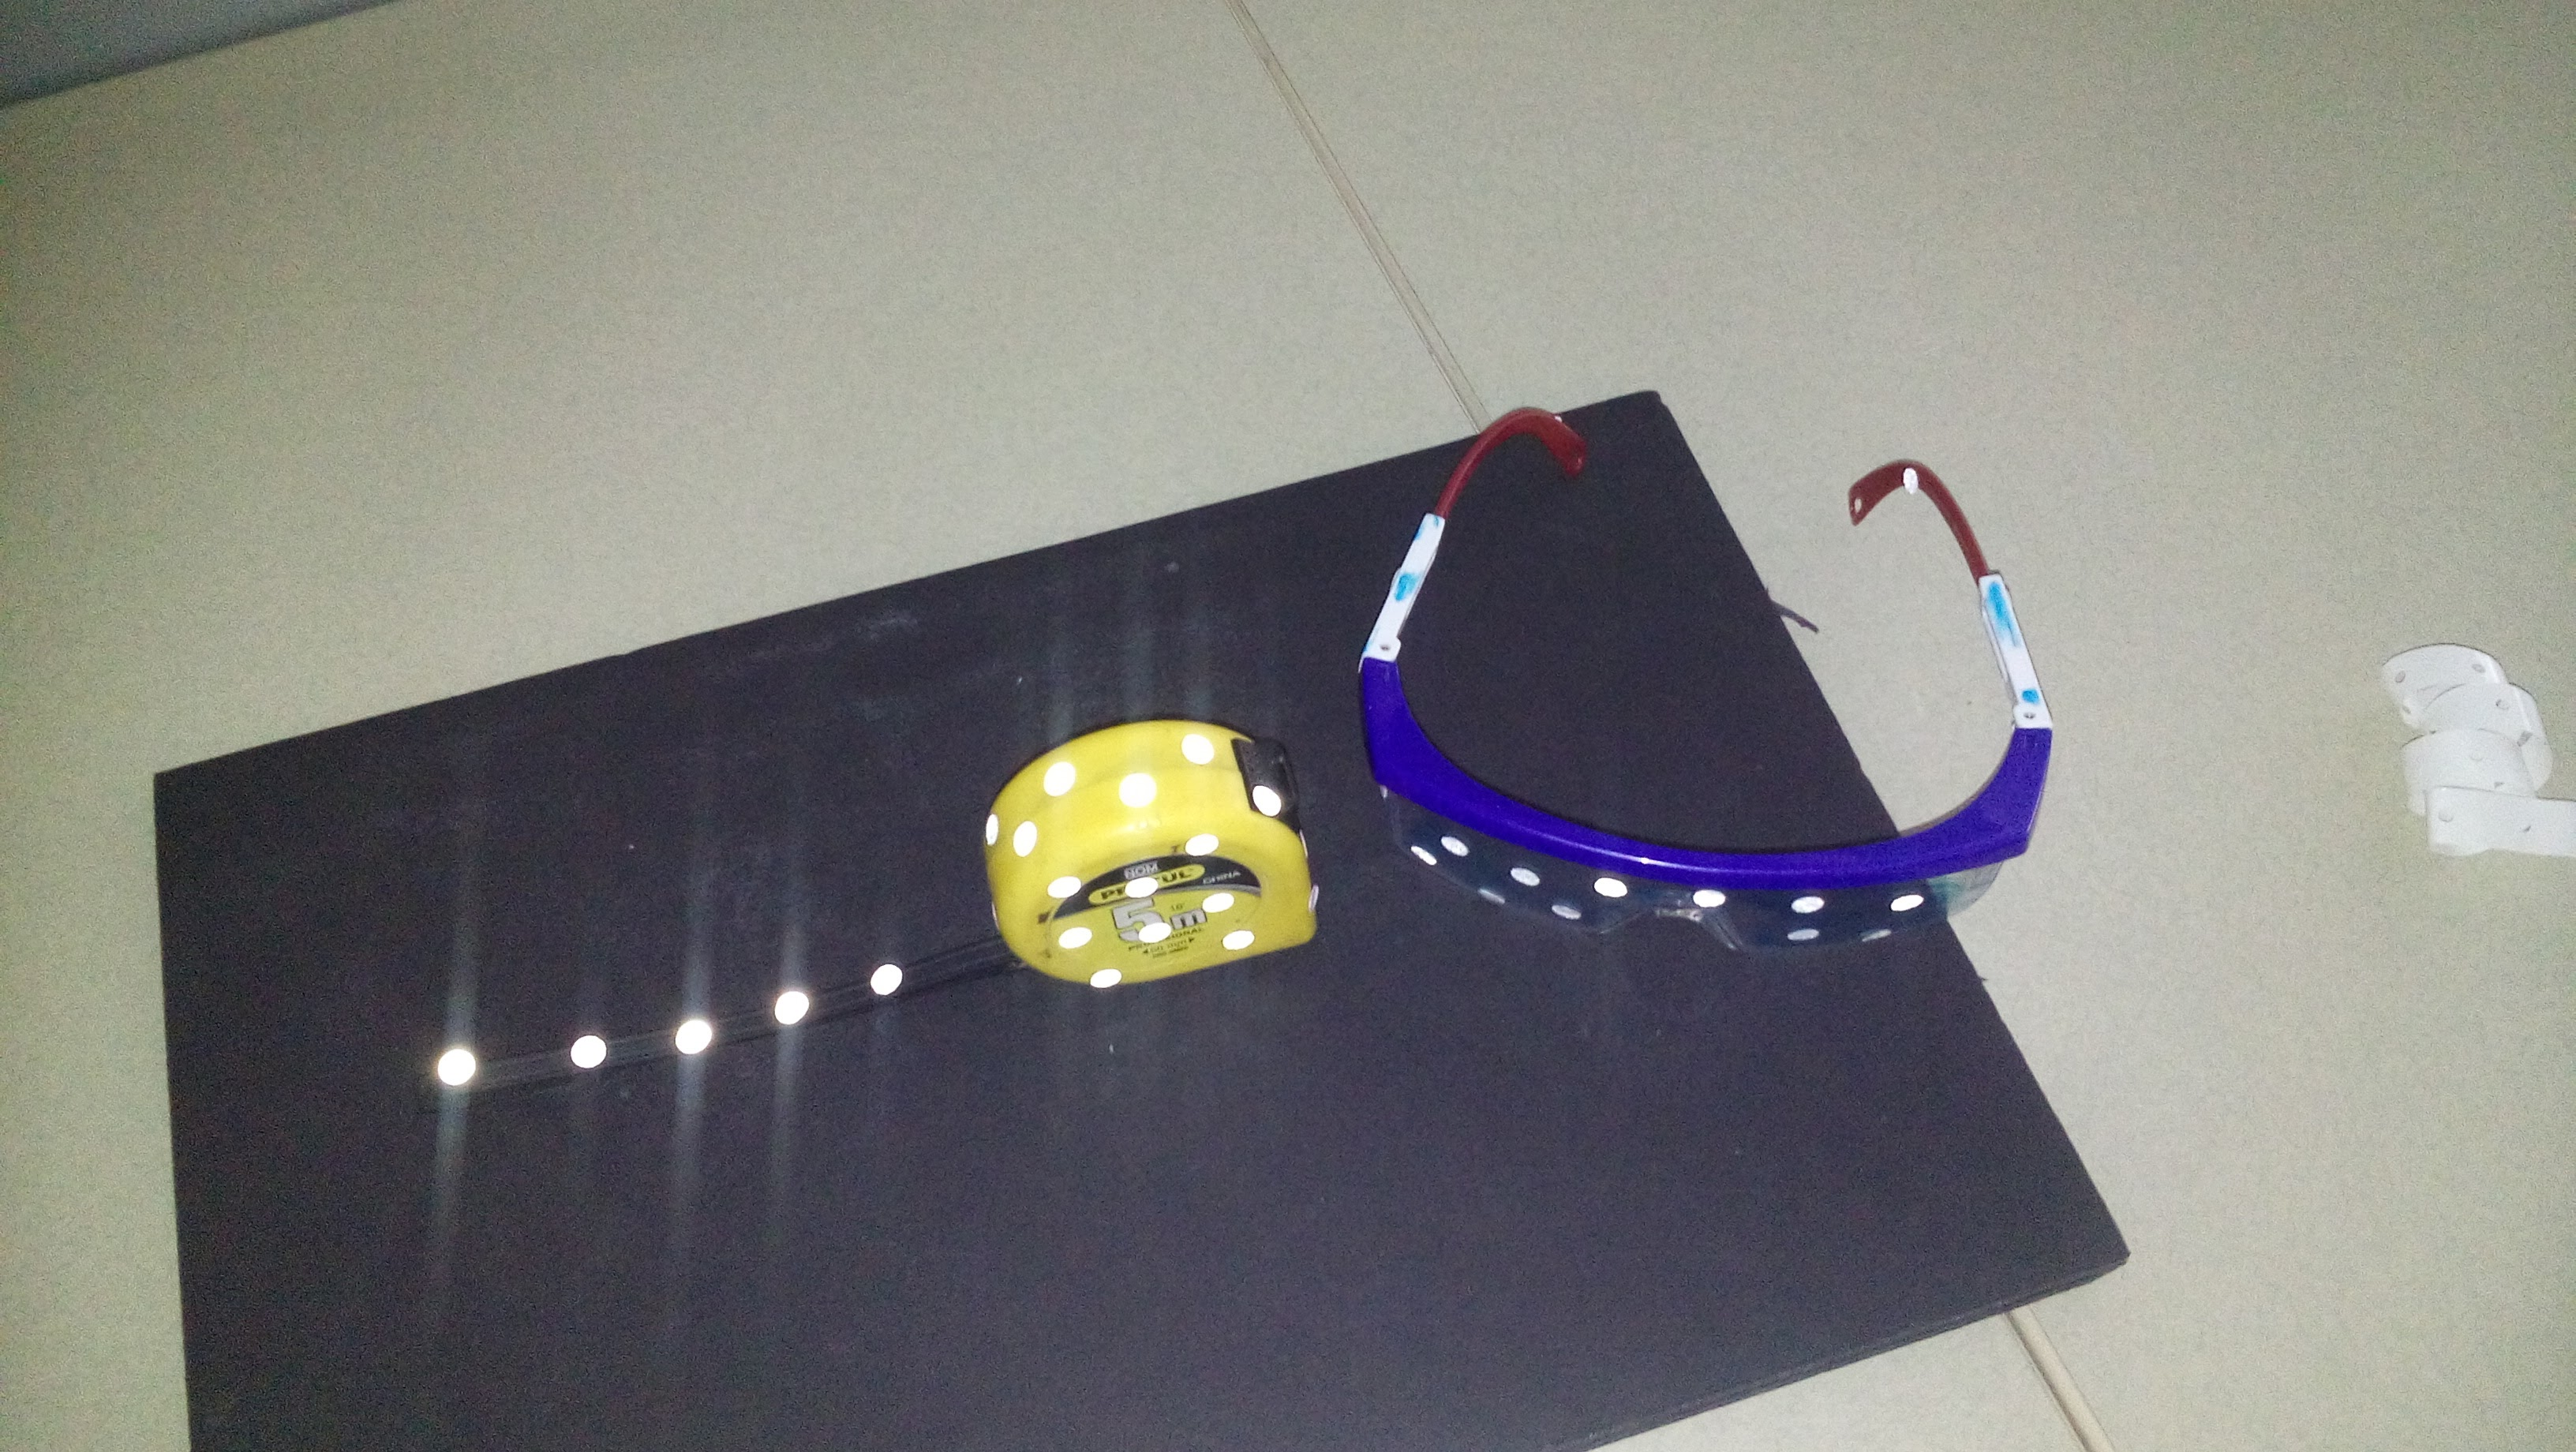
\includegraphics [scale=0.1]
 {./img/20160502_180537.jpg}
  \caption{Preparaci\'on de los objetos a escanear.}
 \end{figure}

 \begin{figure}[!htbp]
 \centering
 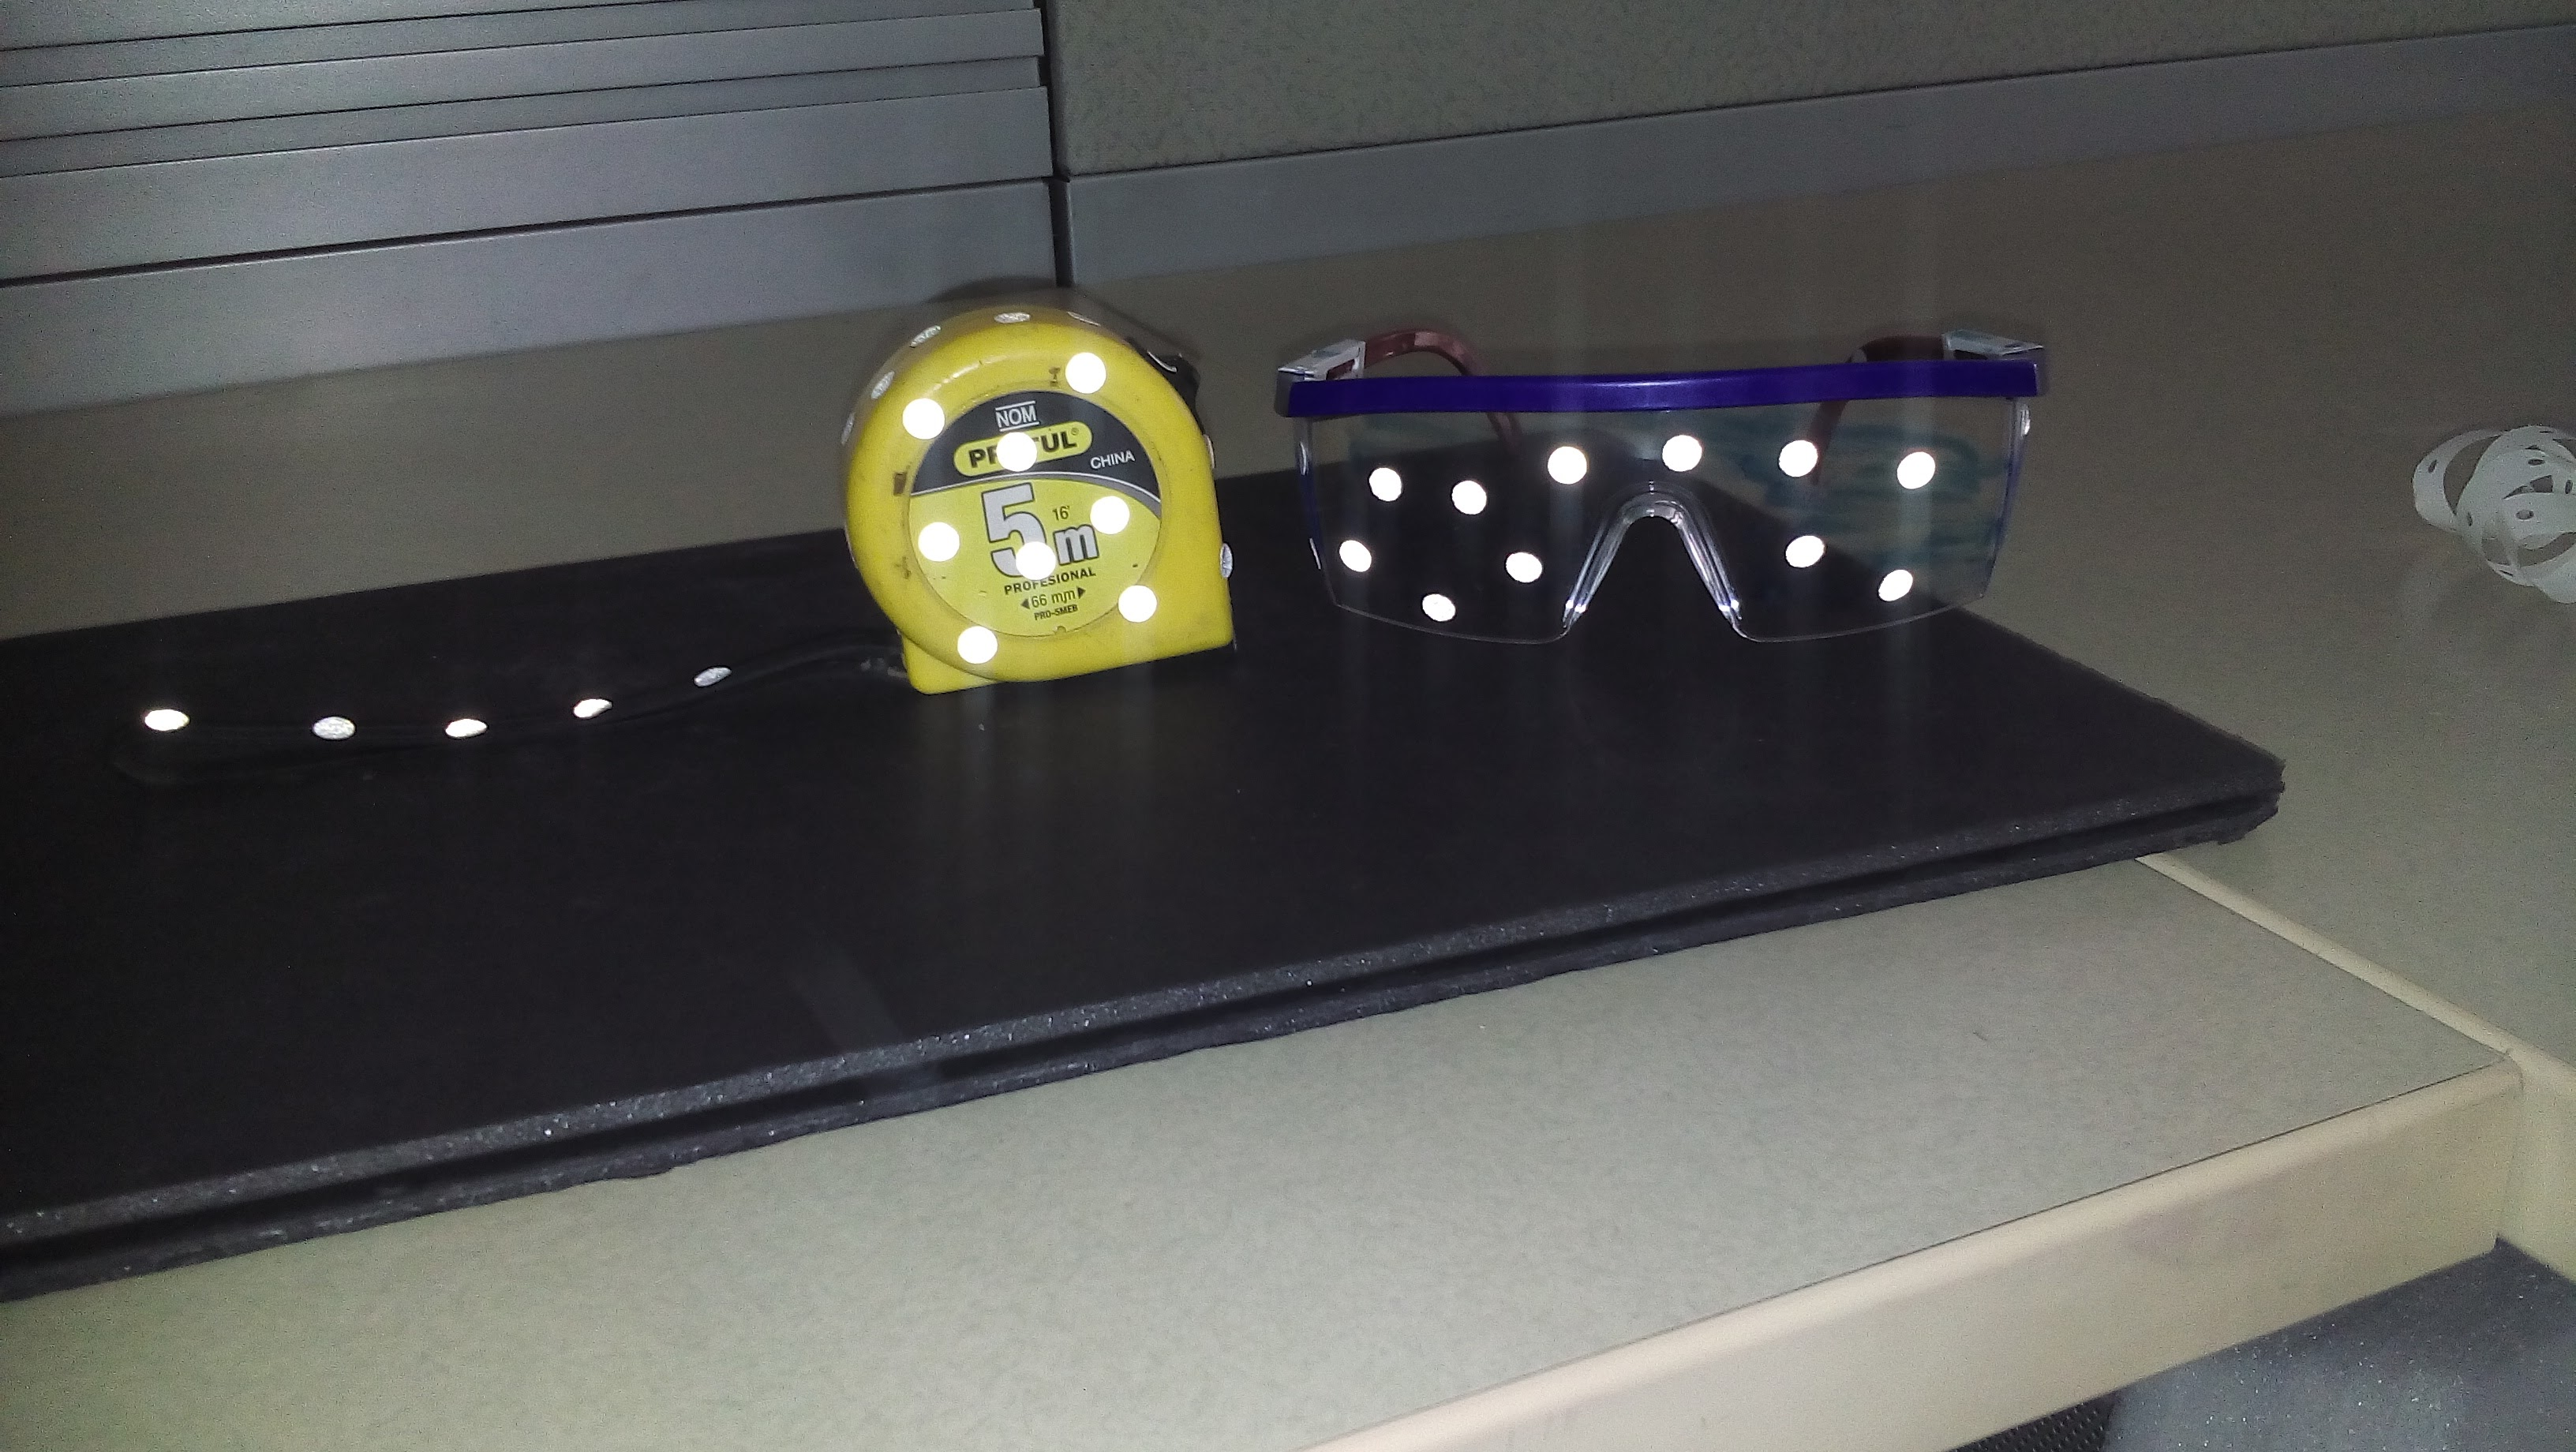
\includegraphics [scale=0.1]
 {./img/20160502_180544.jpg}
  \caption{Objetos a escanear.}
 \end{figure}

 \begin{figure}[!htbp]
 \centering
 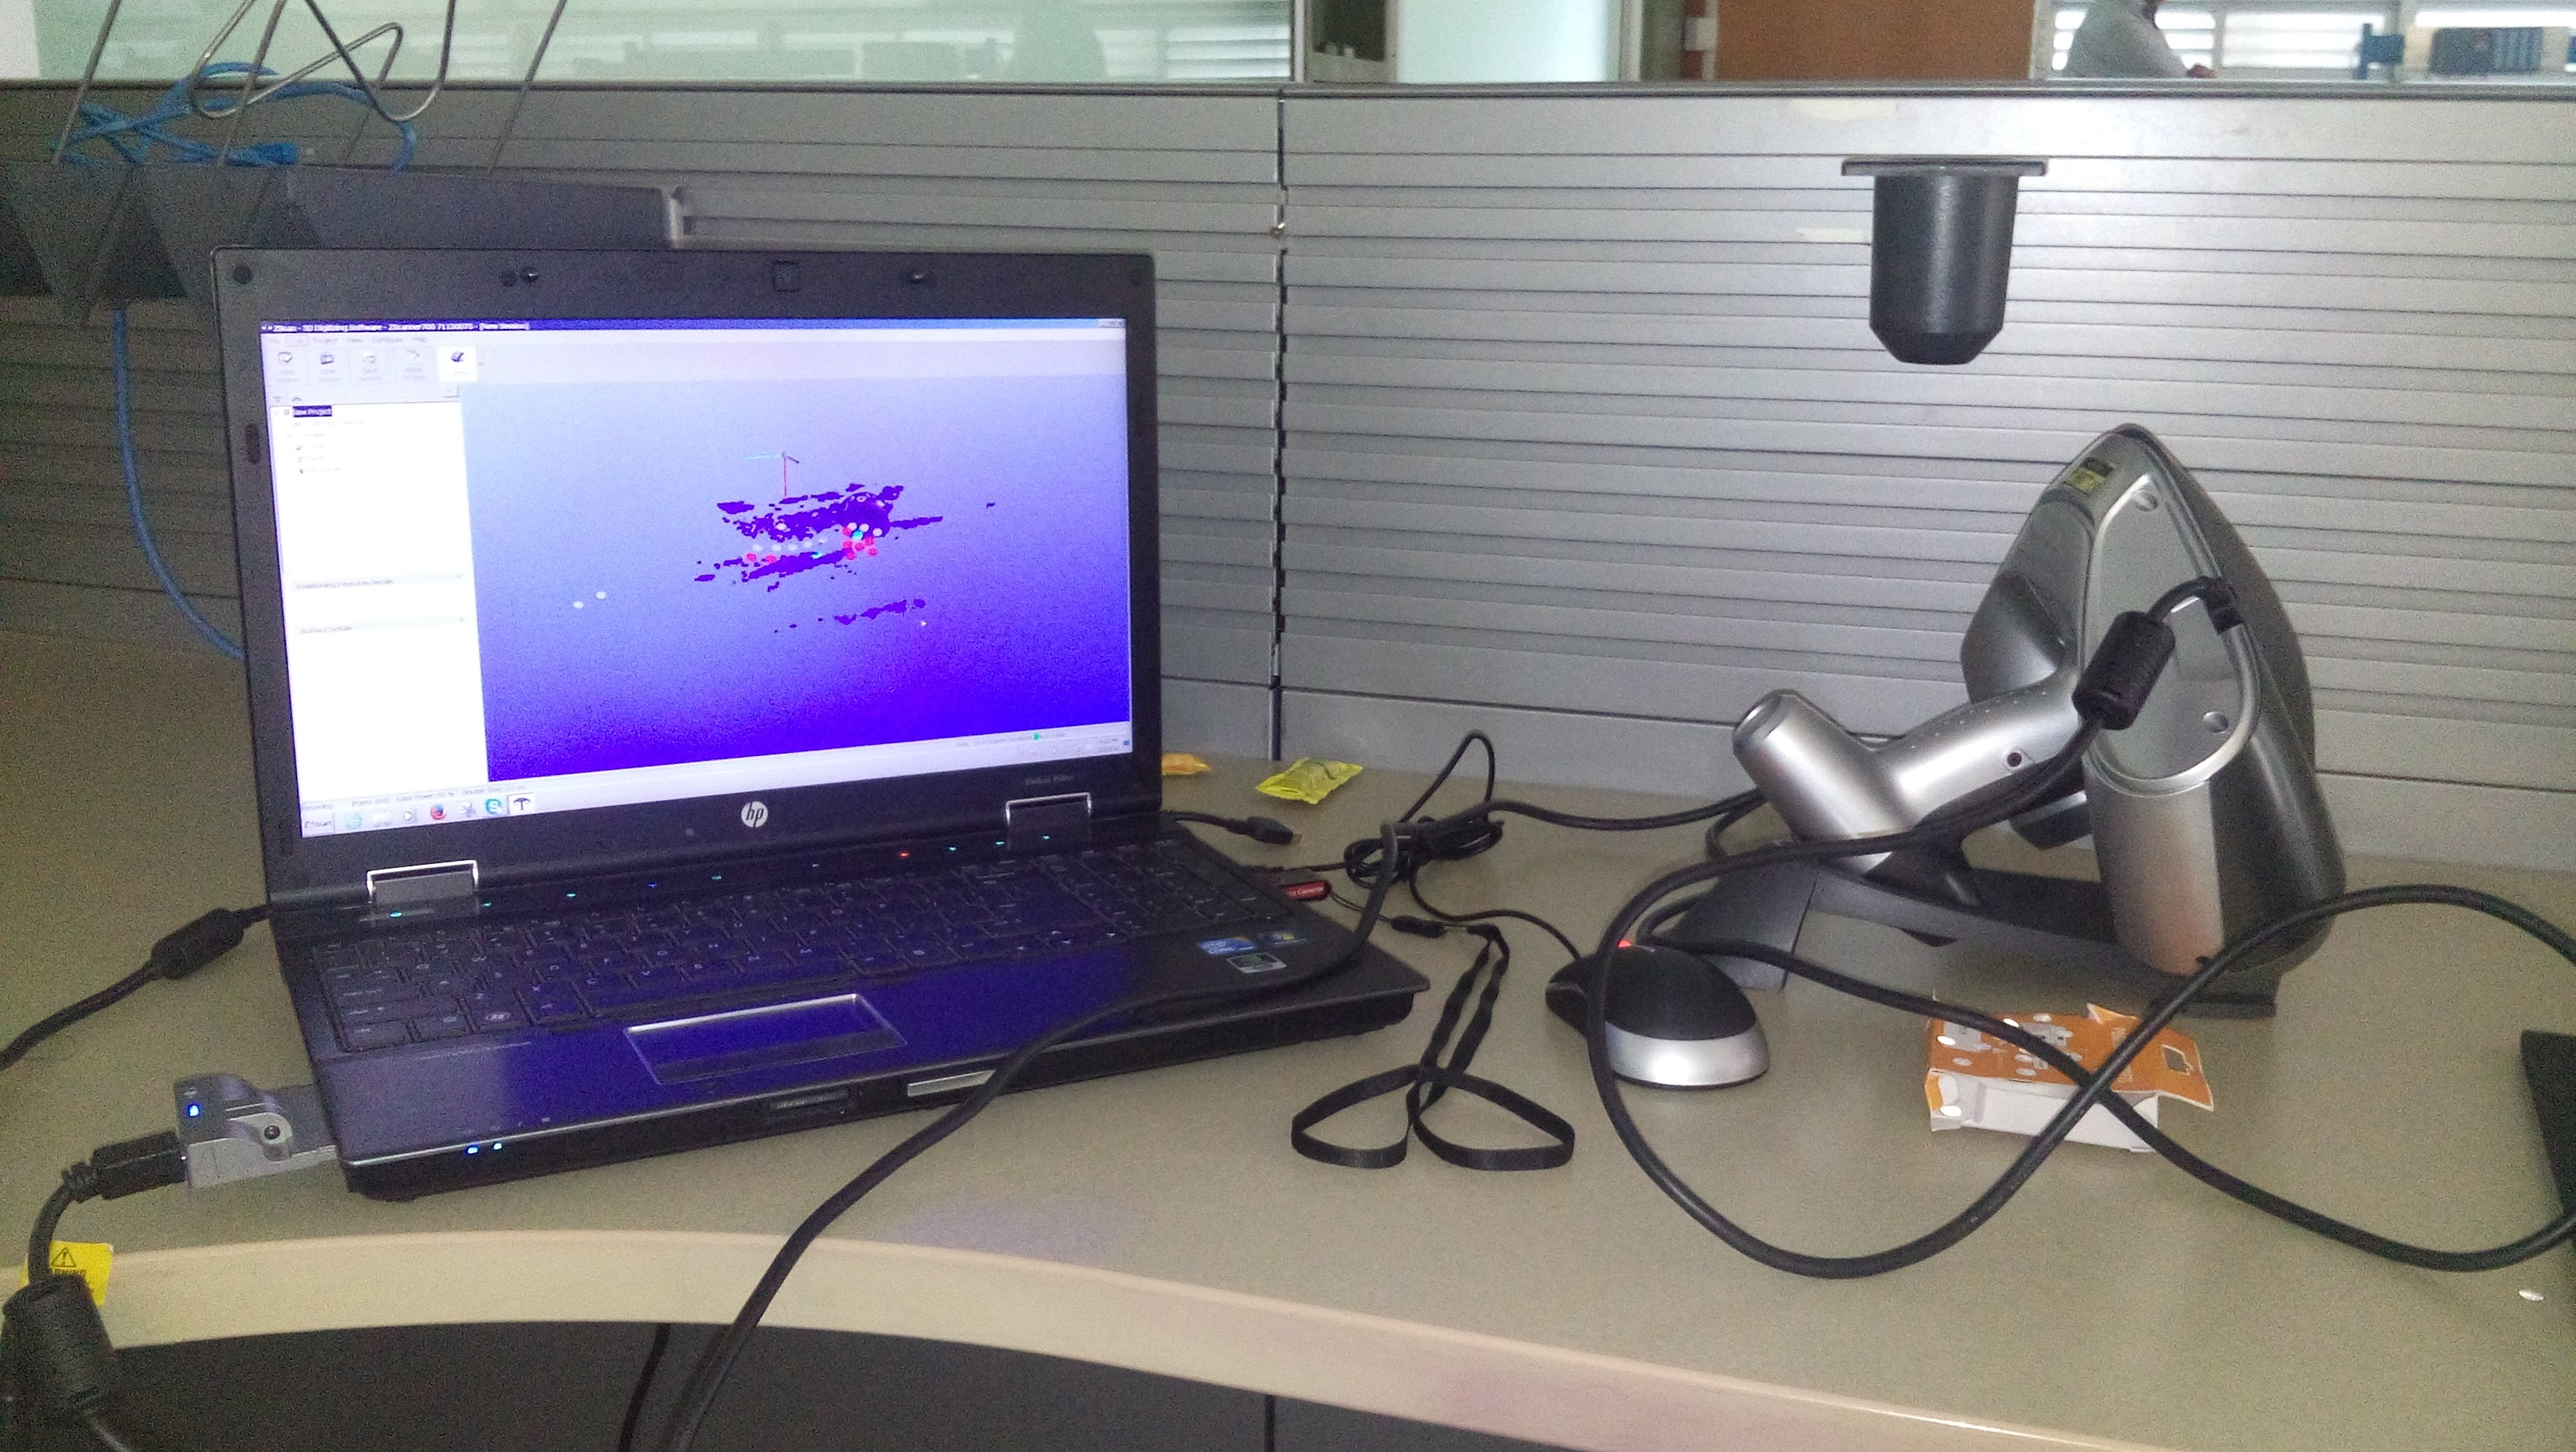
\includegraphics [scale=0.1]
 {./img/20160502_180551.jpg}
  \caption{Material necesario.}
 \end{figure}

  \begin{figure}[!htbp]
 \centering
 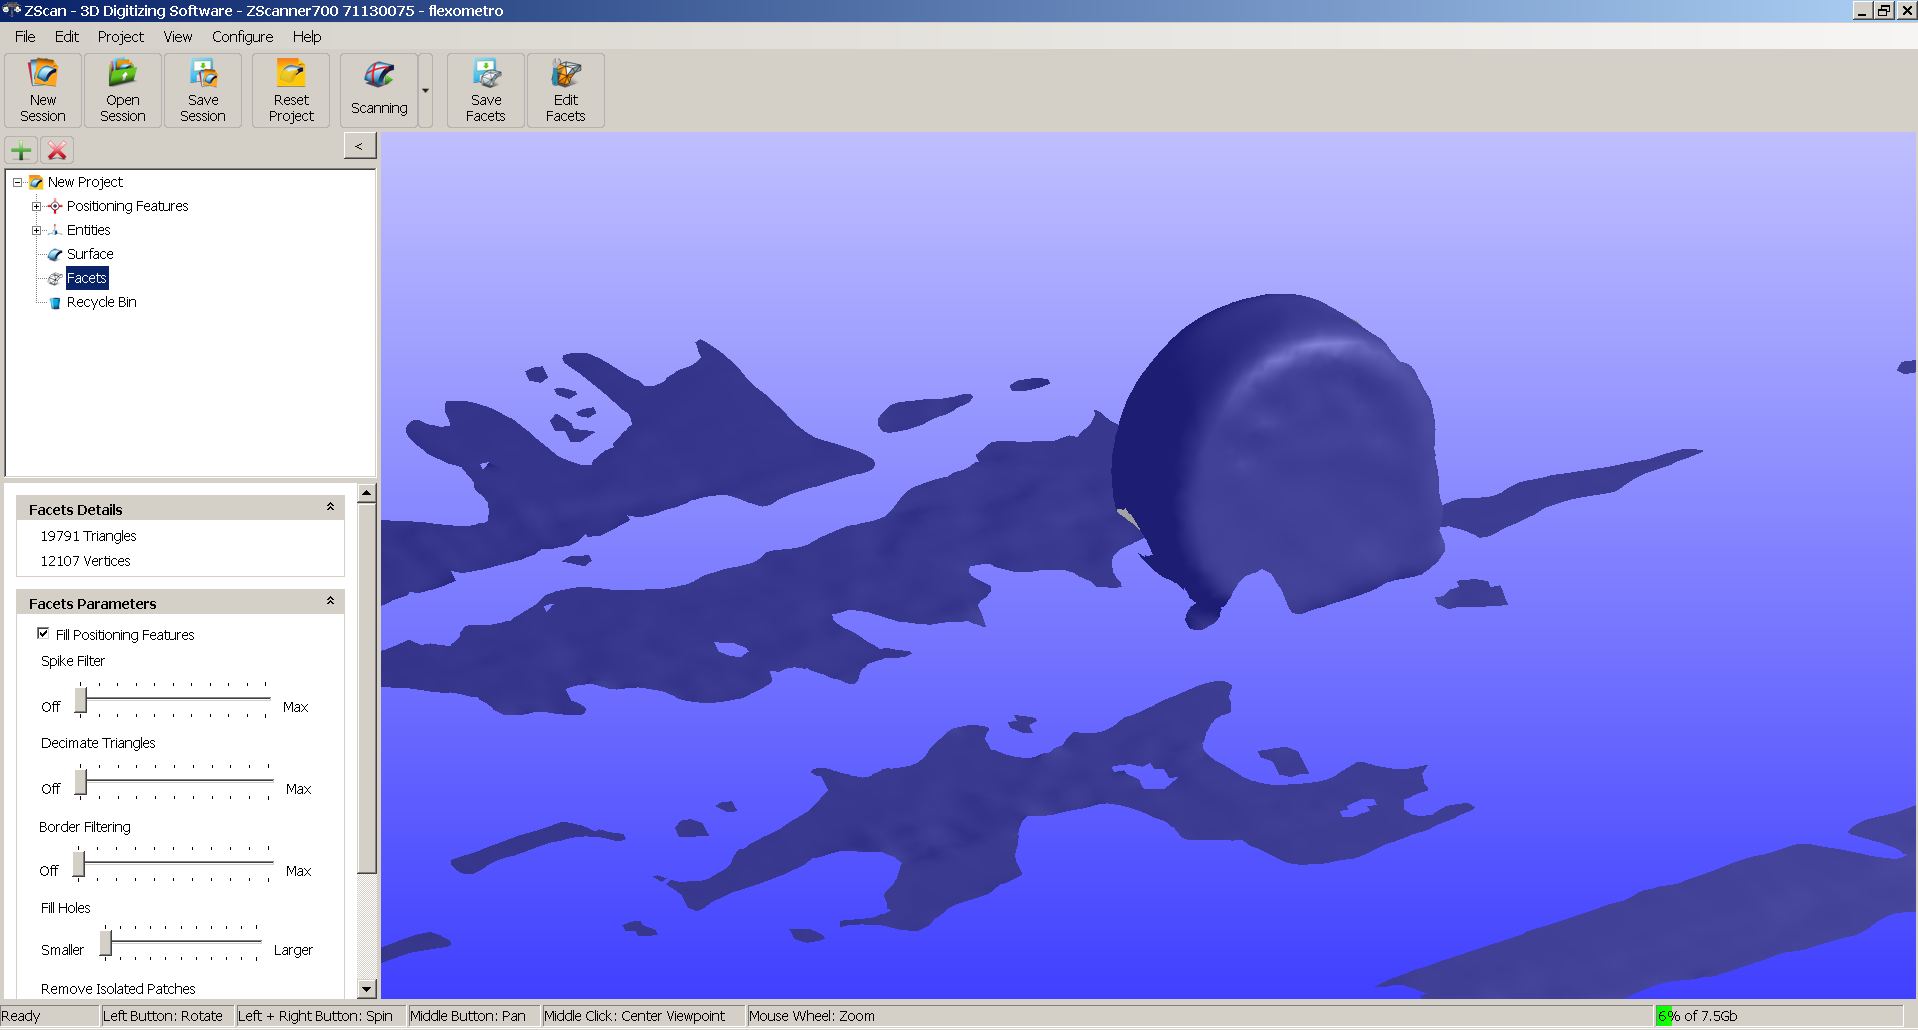
\includegraphics [scale=0.3]
 {./img/flexo_GUI.png}
  \caption{Esc\'aneo del flex\'ometro.}
 \end{figure}

  \begin{figure}[!htbp]
 \centering
 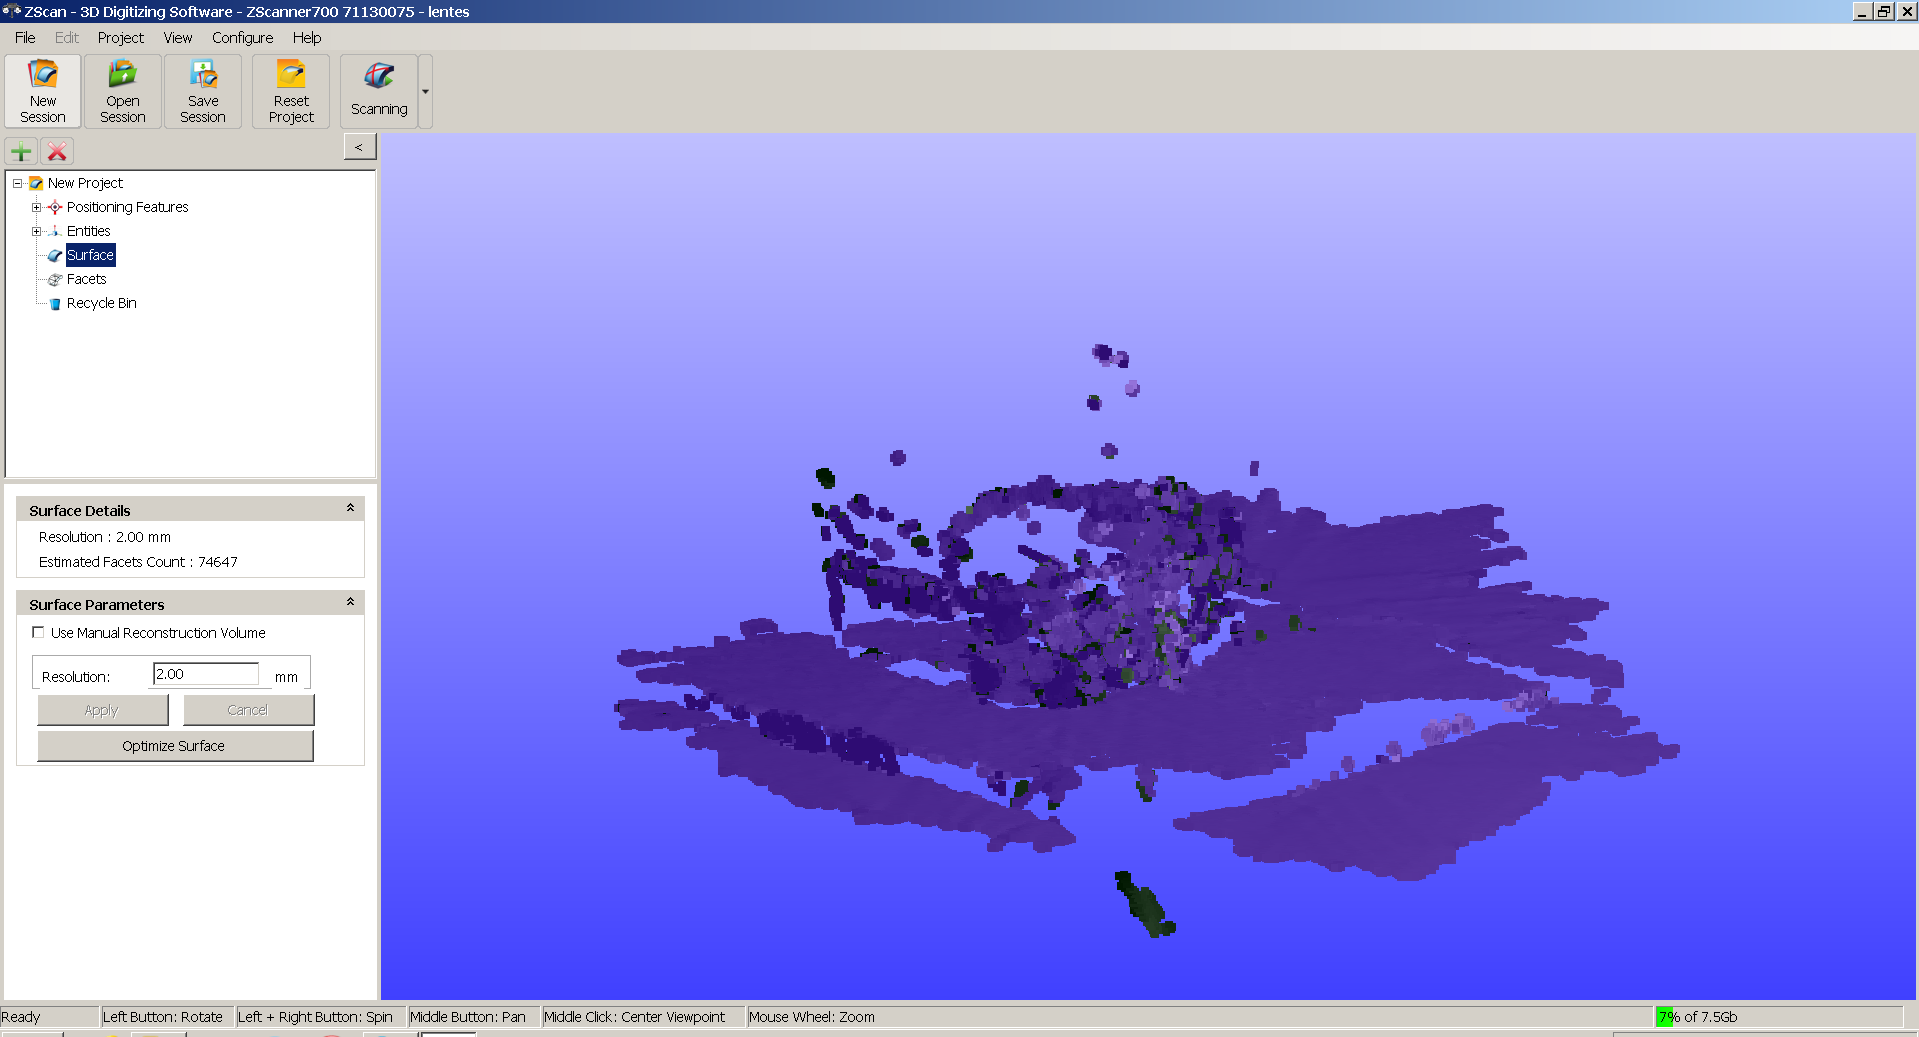
\includegraphics [scale=0.3]
 {./img/lentes_gui.png}
  \caption{Escaneo del par de lentes de seguridad.}
 \end{figure}

 \pagebreak